\documentclass[tikz,border=2pt,11pt]{standalone}
\usetikzlibrary{fit}
\usetikzlibrary{decorations.pathreplacing}
\usetikzlibrary{calc}
\usetikzlibrary{positioning}
\usetikzlibrary{backgrounds}
\usetikzlibrary{arrows.meta}
\usetikzlibrary{matrix}
\usepackage{amsmath}
\usepackage{amssymb}
\usepackage{tikz}
\newcommand{\C}{\mathbb C}
\newcommand{\R}{\mathbb R}
\newcommand{\N}{\mathbb N}
\newcommand{\Id}{I}
\newcommand{\eps}{\varepsilon}
\DeclareMathOperator{\GL}{GL}
\DeclareMathOperator{\Mat}{Mat}
\DeclareMathOperator{\diag}{diag}
\DeclareMathOperator{\rank}{rank}
\DeclareMathOperator{\tr}{tr}
\DeclareMathOperator{\supp}{supp}
\DeclareMathOperator{\nnz}{nnz}
\DeclareMathOperator{\im}{im}
\DeclareMathOperator{\Span}{span}
\DeclareMathOperator{\poly}{poly}
\begin{document}
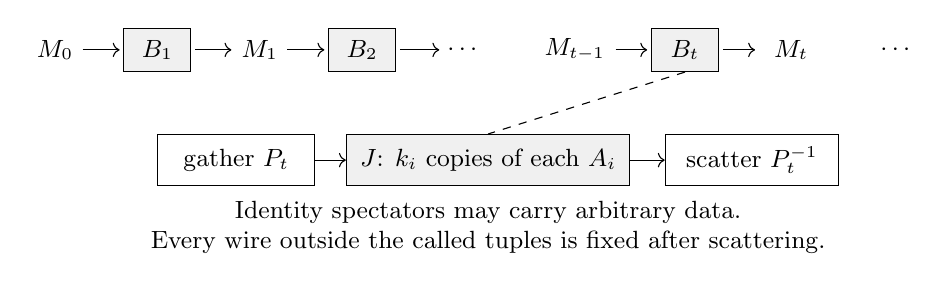
\begin{tikzpicture}[x=1cm,y=1cm, every node/.style={font=\small}]
 \node at (0,1.35) {$M_0$};
 \node[draw,fill=gray!12,minimum width=.85cm,minimum height=.55cm] (b1) at (1.3,1.35) {$B_1$};
 \node at (2.6,1.35) {$M_1$};
 \node[draw,fill=gray!12,minimum width=.85cm,minimum height=.55cm] (b2) at (3.9,1.35) {$B_2$};
 \node at (5.2,1.35) {$\cdots$};
 \node at (6.6,1.35) {$M_{t-1}$};
 \node[draw,fill=gray!12,minimum width=.85cm,minimum height=.55cm] (bt) at (8,1.35) {$B_t$};
 \node at (9.35,1.35) {$M_t$};
 \node at (10.7,1.35) {$\cdots$};
 \draw[->] (.35,1.35)--(.82,1.35);
 \draw[->] (1.78,1.35)--(2.24,1.35);
 \draw[->] (2.95,1.35)--(3.42,1.35);
 \draw[->] (4.38,1.35)--(4.88,1.35);
 \draw[->] (7.12,1.35)--(7.52,1.35);
 \draw[->] (8.48,1.35)--(8.89,1.35);
 \node[draw,minimum width=2cm,minimum height=.65cm] (g) at (2.3,-.05) {gather $P_t$};
 \node[draw,fill=gray!12,minimum width=3.6cm,minimum height=.65cm] (j) at (5.5,-.05) {$J$: $k_i$ copies of each $A_i$};
 \node[draw,minimum width=2.2cm,minimum height=.65cm] (s) at (8.85,-.05) {scatter $P_t^{-1}$};
 \draw[->] (g.east)--(j.west);
 \draw[->] (j.east)--(s.west);
 \draw[dashed] (bt.south)--(j.north);
 \node[align=center] at (5.5,-.9) {Identity spectators may carry arbitrary data.\\
 Every wire outside the called tuples is fixed after scattering.};
\end{tikzpicture}
\end{document}
